\documentclass[12pt]{article}
\usepackage[utf8]{inputenc}
\usepackage[top=0.75in, bottom=0.5in, left=0.5in, right=0.5in]{geometry}
\usepackage{amssymb}
\usepackage{tabu}
\usepackage{array}
\usepackage{indentfirst}
\usepackage{fancyhdr}
\usepackage{lastpage}
\usepackage[usenames, dvipsnames]{color}
\usepackage{graphicx}
\usepackage{pdfpages}
\usepackage{placeins}
\usepackage{titlesec}
\usepackage{paralist}
\usepackage[dvipsnames]{xcolor}
\usepackage{wrapfig}


\titleformat*{\section}{\Large\bfseries}
\titleformat*{\subsection}{\large\bfseries}
\titleformat*{\subsubsection}{\small\bfseries}
\titlespacing*{\section}
{0pt}{2.ex plus 1ex minus 2.0ex}{1.3ex plus .2ex}
\titlespacing*{\subsection}
{0pt}{2.ex plus 1ex minus 2.0ex}{1.3ex plus .2ex}
\pagestyle{fancy}
\fancyhf{}
\rhead{Page \thepage \hspace{1pt} of \pageref{LastPage}}
\lhead{Zhelun Zhang zz84, Yixin Shi ys447, Yuanxi Shen ys448}
\setlength{\parindent}{1em}
\renewcommand{\baselinestretch}{1}
\title{\vspace{-2.0cm}Movie Rating Prediction}
\date{\vspace{-13ex}}
\begin{document}

\maketitle
\thispagestyle{fancy}
\section{The Dataset}
\subsection{Description}
There are in total 7 CSV files in provided ``Movies Dataset". We first take a closer look at the ``movies\_metadata.csv" file, since this file provides more comprehensive information of a movie. Namely, this file contains all the basic information, such as production company, budget etc, of a movie. There are approximately 45.5k data points and 24 columns in this dataset. Among these 24 columns, there are two columns named ``vote\_average" and ``vote\_count", where these are correspondingly the \textbf{score} given by reviewers and the \textbf{number of reviewers} for each movie. This is the ``target" for this model.
\subsection{Messy}
This dataset is messy. Three of the 24 columns have more than 50\% of the data is missing (not counting zeros values, which are sometimes not informative). The rest of columns are as well complicated. \par Take our target, vote\_average for example, even though there are only 6 missing data, there are approximately 3000 data points that has value zero. Even though the data is not missing, this does not provide much information. A histogram given by Kaggle is shown below on the left:
\begin{wrapfigure}{L}{0.4\textwidth}
\centering
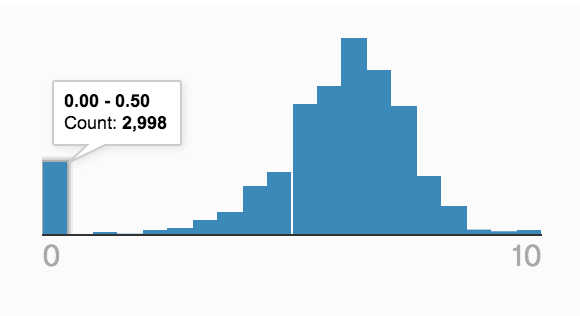
\includegraphics[width=0.4\textwidth]{voteAverage.png}
\caption{Vote\_Average}
\end{wrapfigure}\par
As we can see, there are 2998 data points that has 0 value for vote\_average. If we ignore the 0 values, we observe that the rest of the scoring is approximately Gaussian. Hence, we can see that we should also be dealing with zero values besides missing data. Similar situations can be observed in other columns. 
\section{Features and Preprocessing}
\subsection{Features Considered}
Among the 24 columns, we only pick a portion of features we want to taken into consideration at this point. Our first choice is numerical data. The six main features we taken into consideration is \textbf{Budget, Popularity, Release Date, Runtime, Genres, Production Countries}. We have also considered \textbf{Production Company}. However, we observe that there are too many categories existing, which makes the matrix large and sparse, not useful when doing Linear Regression.
\subsection{Preprocessing}
There are two main parts in preprocessing process. One is to solve the problem of ``messy"; the other is to encode.
\begin{itemize}
    \item \textbf{Genre} We parse the given Genre information from JSON to string. After that, we use \textcolor{purple}{many-hot encoding} to process Genre information. The reason for such encoding is because each movie can belong to several categories.
    \item \textbf{Popularity: Float} The Popularity information is given by the dataset. It is given as a float type, so we can directly parse the data. For those missing data, we replace them with 0.
    \item \textbf{Budget} For budget feature, we use \textcolor{purple}{Boolean encoding}. By observing data, we set three ``levels" of budget: [0, 1, 20] $\times10^6$ (dollars). For the mismatched and missing values, we replace them with 0, since we are not able to give any predictions.
    \item \textbf{Runtime} For runtime of a movie, we also use \textcolor{purple}{Boolean encoding}. We compute 25\%, 50\%, 75\% quantiles, and use these values as reference when doing Boolean encoding. For missing value and zero value, we set them to the mean value to reduce variance.
    \item \textbf{Release Date} For release date of a movie, we only care which months are the movies released.We use \textcolor{purple}{one-hot encoding} on month/quarter. For missing values, we randomly assign a month to it.
    \item \textbf{Production Countries} There are many countries included. We first tried a \textcolor{purple}{many-hot encoding}, but was not succesful. A quick examination into the Production Countries feature reveals to us that among the 45.5k movies, 21.1k of them are produced in the US. So, we replace this feature with a single vector indicating whether the movie is produced in the US.
\end{itemize}
\subsection{Preprocessing $y$ target}
\begin{wrapfigure}{R}{0.25\textwidth}
\centering
\includegraphics[width=0.25\textwidth]{single1.png}
\caption{Single Feature}
\end{wrapfigure}\par
To avoid useless movie ratings, we use the IMDB's weighted rating formula:
Weighted Rating (WR) = ($\frac{v}{v+m}\times R + \frac{m}{v+m}\times C$)
, where $v$ is the number of votes for the movie, $m$ is the minimum votes required to be listed in the chart, $R$ is the average rating of the movie, $C$ is the mean vote across the whole report.

The next step is to determine an appropriate value for m, the minimum votes required to be listed in the chart. We will use 95th percentile as our cutoff. In other words, for a movie to feature in the charts, it must have more votes than at least 95\% of the movies in the list.
\section{Linear Models}
\subsection{Prevent Overfitting}
We split our dataset into train, validate, test parts, with portion 7:2:1. Before we test our output, we validate our model with validation set to prevent overfitting. That is, validation error is slightly bigger than training error; while both of them are relatively low. \begin{wrapfigure}{L}{0.25\textwidth}
\centering
\includegraphics[width=0.25\textwidth]{single2.png}
\caption{Single Feature}
\end{wrapfigure}\par We also use random seed, and shuffle our data before splitting.
\subsection{Single Feature} We tried 5 out of 6 main feature individually to see which feature is most effective in predicting via Linear regression. We use \textbf{MSE} as our error metric. The result are shown in Figure 2 and Figure 3.
By observation, we see that \textbf{Popularity} has the smallest MSE error. This indicates that Popularity it the starting point we want to pick. 
\subsection{Three Models}
We plotted the data points \textbf{linear, quadratic, and cubic} with respect to $y$ and see that Popularity and y is NOT simply linearly related. In fact, quadratic and cubic models, or even quartic model, might give better linear regression results. As follows, we fit all of them to see which has the smallest validation error. We find that \textbf{cubic} model has the least MSE error, and the fitting is shown below in Figure 4.
\par The validation error is 3.7751873539057144, much smaller than single feature fitting, and still in a good range. We call this \textbf{cubic Popularity Model}. Now we add more features to Popularity and see whether there are some improvements.
\subsubsection{Model I: Popularity, Budget, Runtime, Release Date}
After a few tryouts, we figure out a first model that works better than cubic Popularity Model. When adding more features, we observe some small progress regarding the MSE error metric. 
\begin{wrapfigure}{L}{0.3\textwidth}
\centering
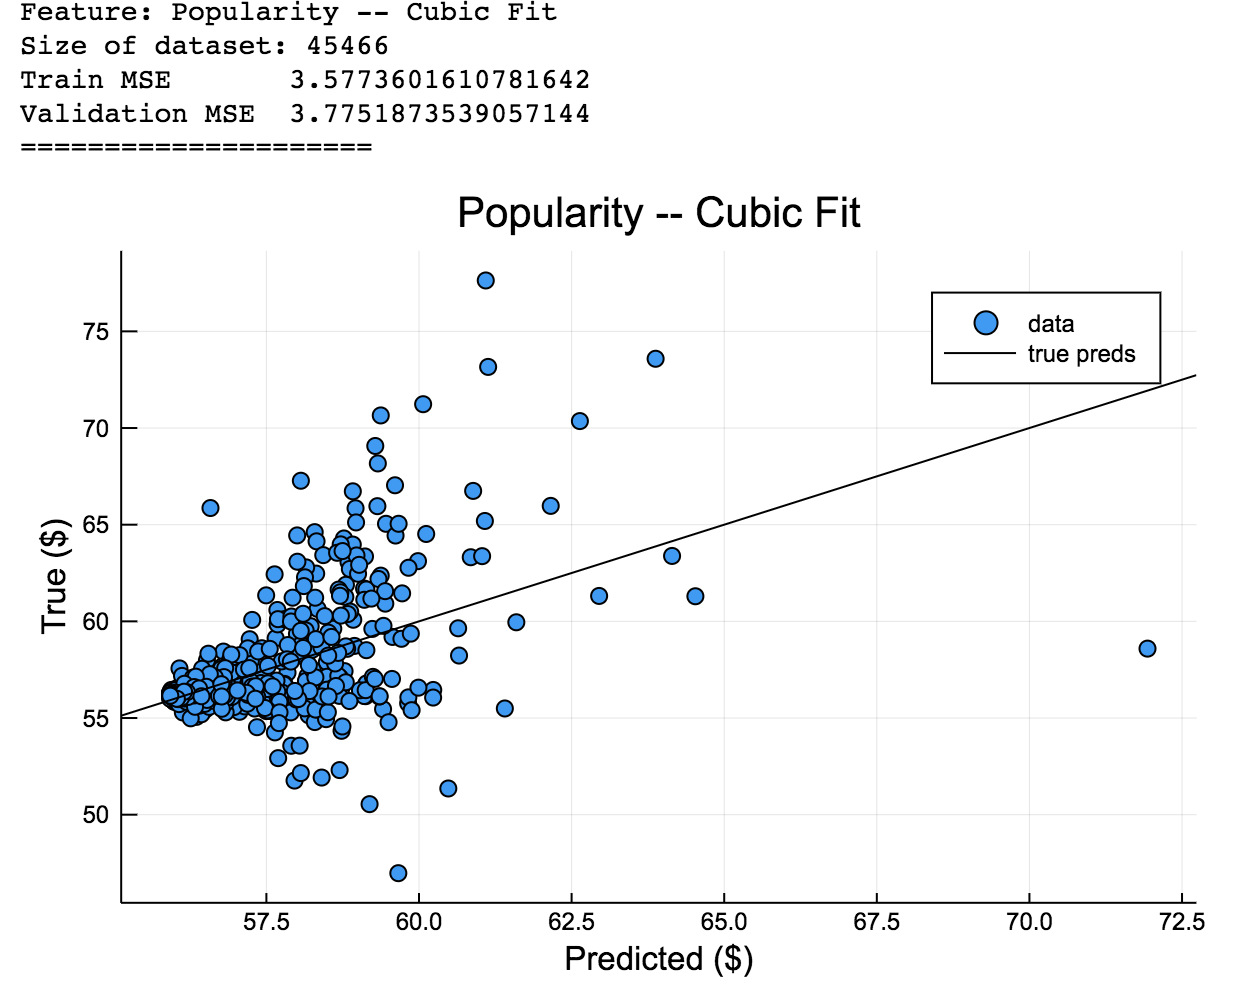
\includegraphics[width=0.3\textwidth]{popularitycube.png}
\caption{Single Feature}
\end{wrapfigure}\par
We now have a tentative \textbf{\textcolor{red}{Model I}}, which includes \fbox{cubic Popularity}, \fbox{(linear) budget, (linear) date}. The resulting plot is shown in Figure 5. The validation error for Model I is 3.674248342579983, which is smaller than cubic Popularity Model.\par We can actually add a little complexity in this model. We do a \textbf{pseudo-polynomial fitting} for Budget and Popularity. The choice of these two features are decided based on a bunch of experiments of several combinations. The reason we call it ``pseudo" is because we only include a portion of polynomial fitting features, but exclude features such as ``budget$^3$". We call this \textbf{\textcolor{red}{Model I Beta}}. The validation error is 3.572925452106735. A lot better!
\subsubsection{Model II and III:}
Model II (and Beta) and Model III (and Beta)are both extensions of Model I (and Beta) adding different features. \textbf{\textcolor{red}{Model II}} is Model I + Production Countries, \textbf{\textcolor{red}{Model II Beta}} is Model I Beta + Production Countries; \textbf{\textcolor{red}{Model III}} and \textbf{\textcolor{red}{Model III}} are Model I adding Genre feature. The resulting plots are shown below. \par Note that the validation error is smaller than the training error in Model III and Model III Beta. This is possibly because there is a few big outliers existent in the training set, and these two models happen to capture these outliers. The outliers are probably in Genres feature, because Model III and III Beta differ from previous models particularly by adding in Genres.
\begin{figure}[h]
   \begin{minipage}{0.3\textwidth}
     \centering
     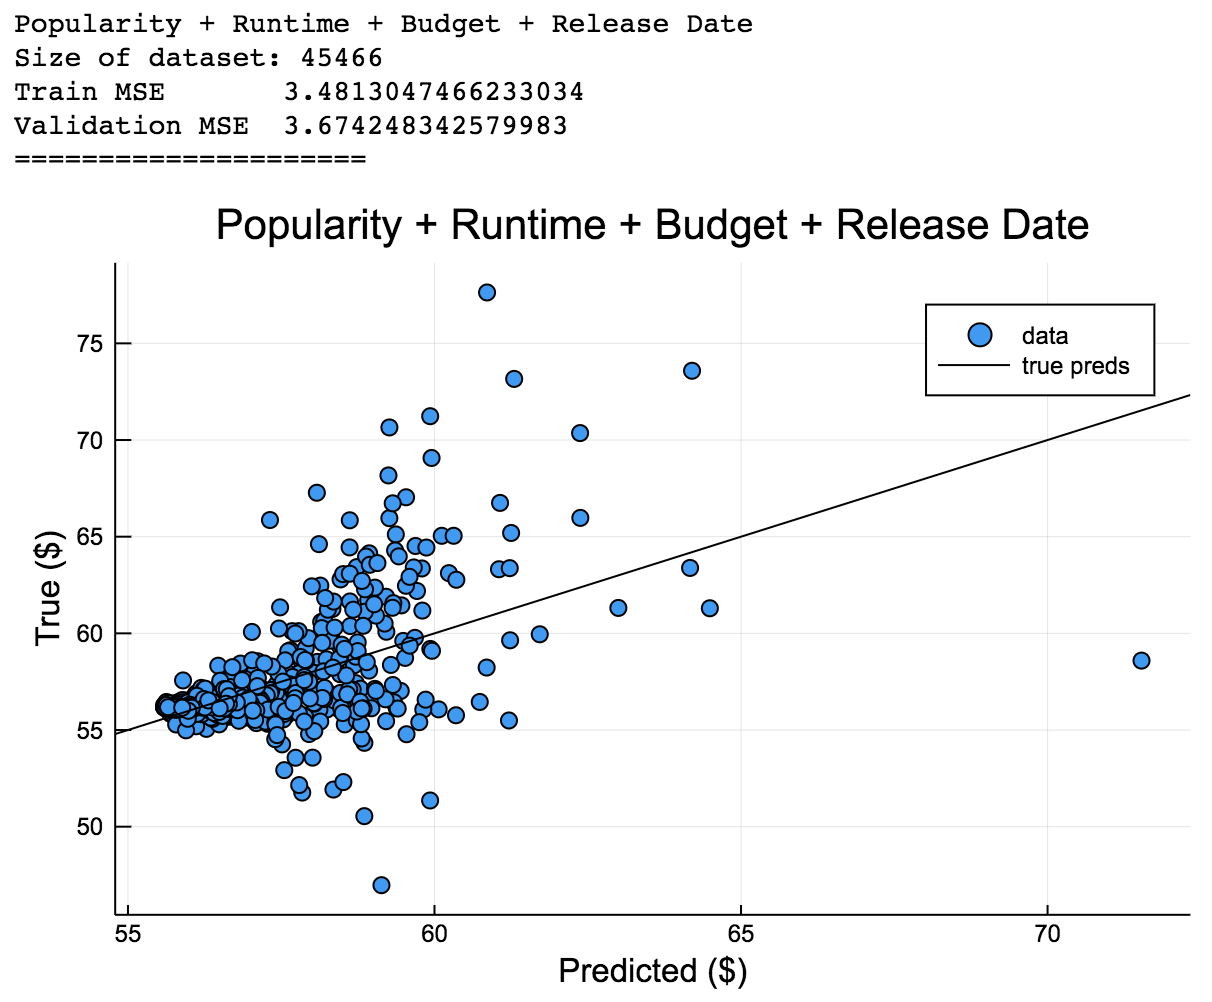
\includegraphics[width=.7\linewidth]{model1.png}
     \caption{Model 1}
   \end{minipage}
   \begin{minipage}{0.3\textwidth}
     \centering
     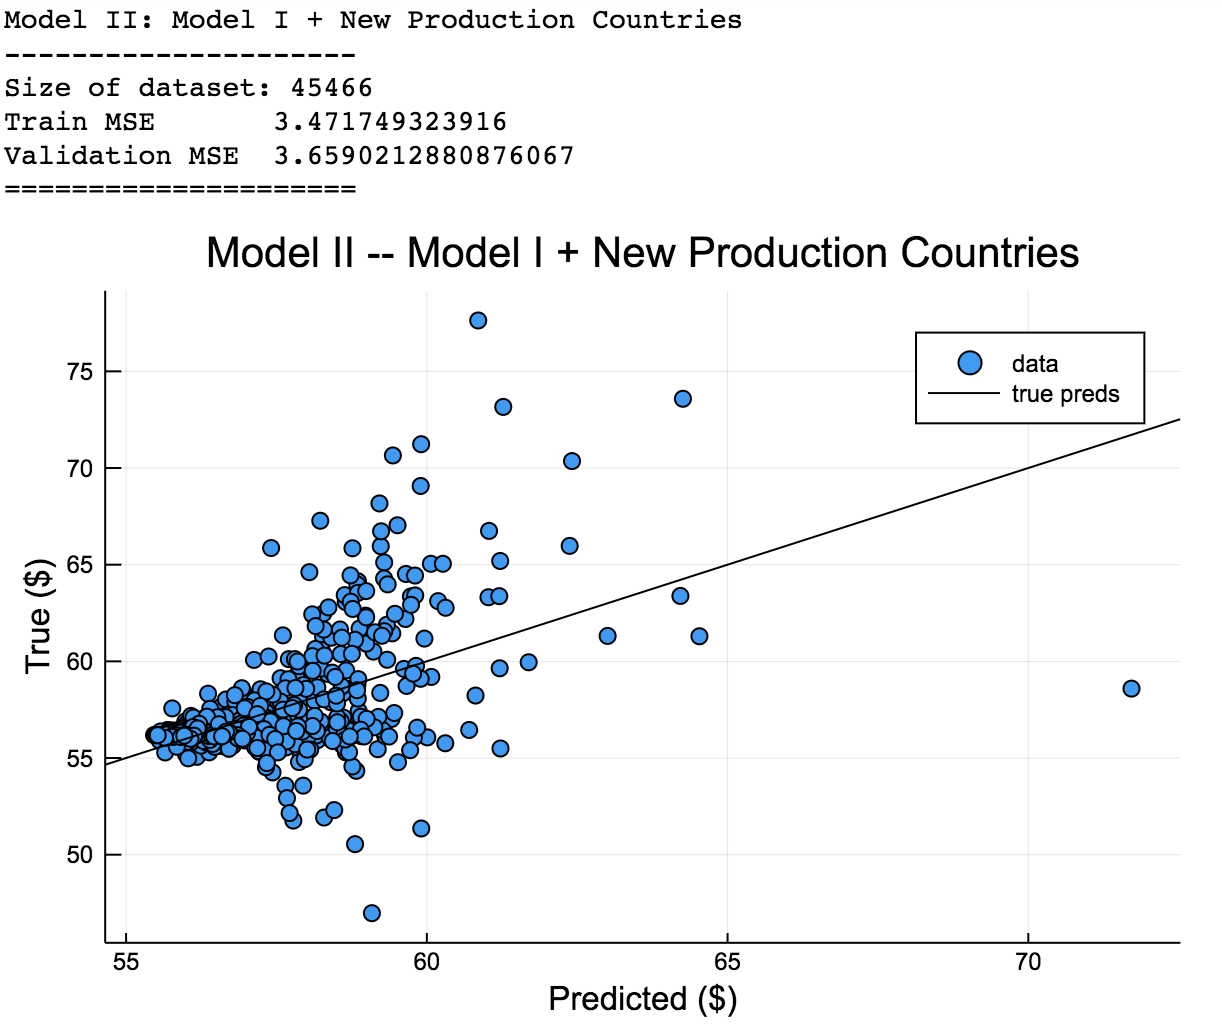
\includegraphics[width=.7\linewidth]{model2.png}
     \caption{Model 2}
   \end{minipage}
%   \begin{minipage}{0.182\textwidth}
%      \centering
%      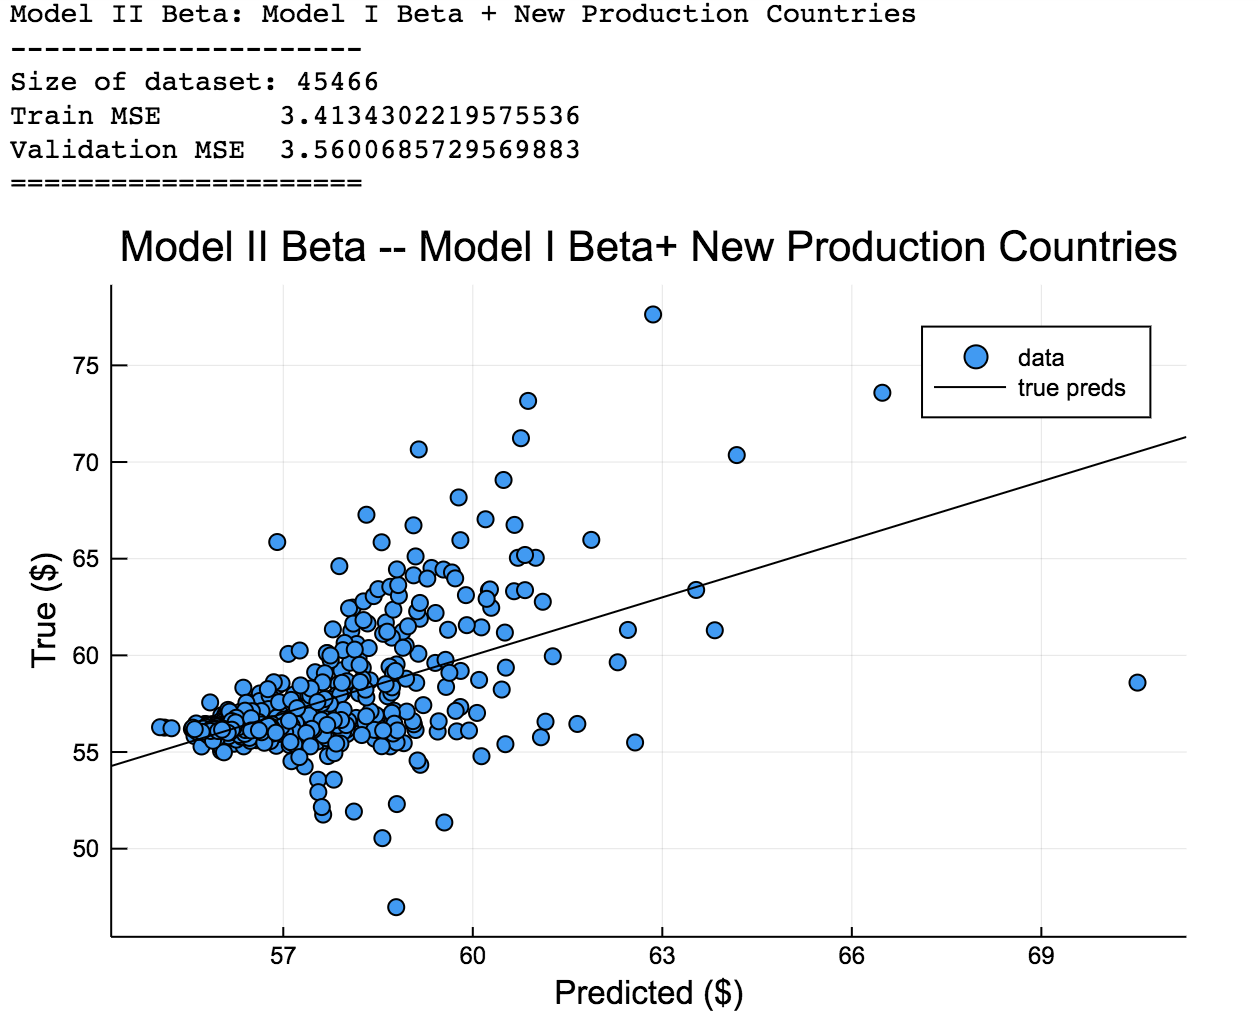
\includegraphics[width=.9\linewidth]{model2beta.png}
%      \caption{Model 2 Beta}
%   \end{minipage}
   \begin{minipage}{0.3\textwidth}
     \centering
     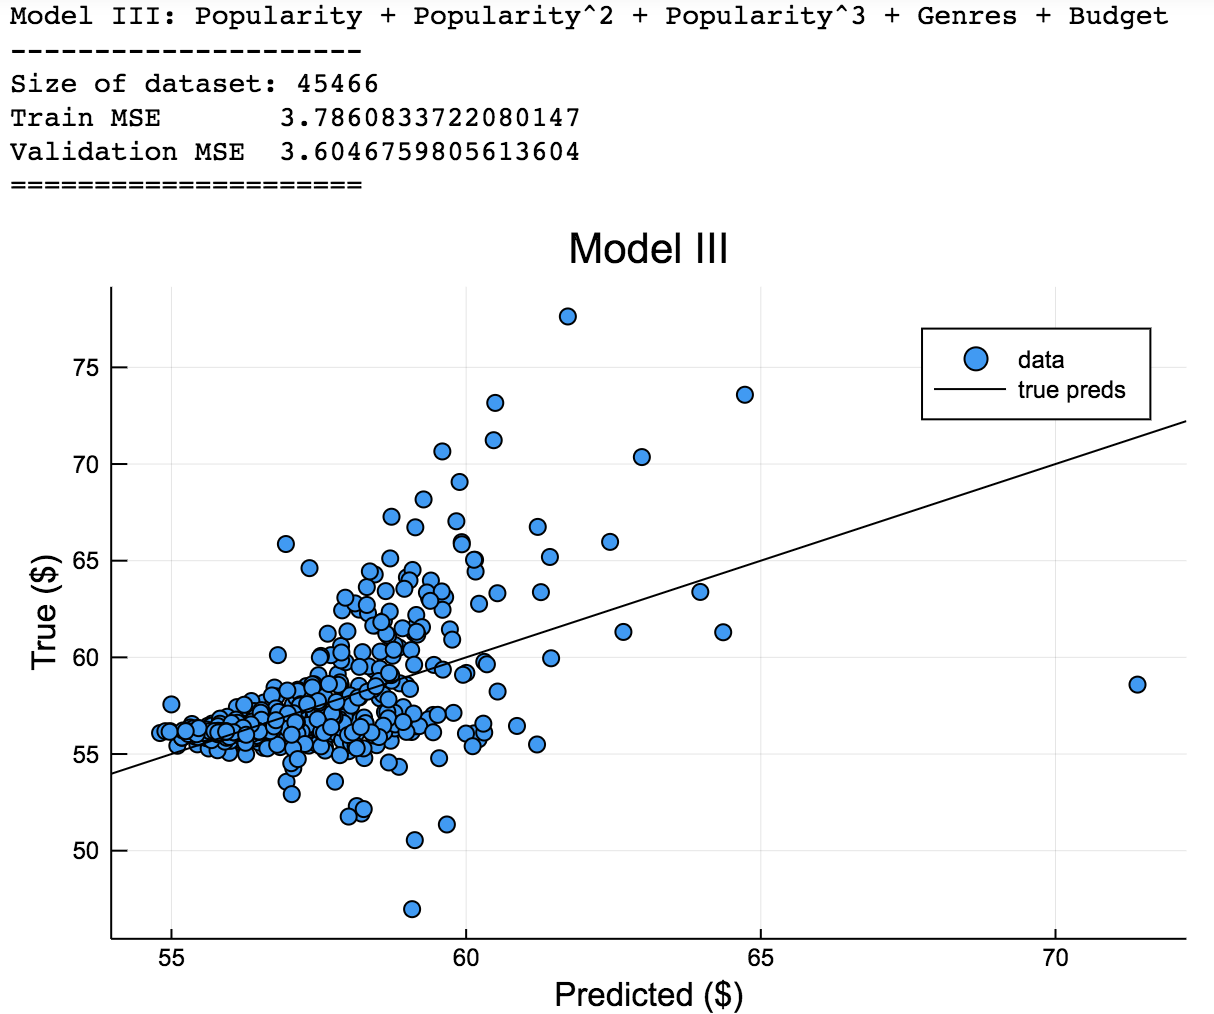
\includegraphics[width=.7\linewidth]{model3.png}
     \caption{Model 3}
   \end{minipage}
%   \begin{minipage}{0.182\textwidth}
%      \centering
%      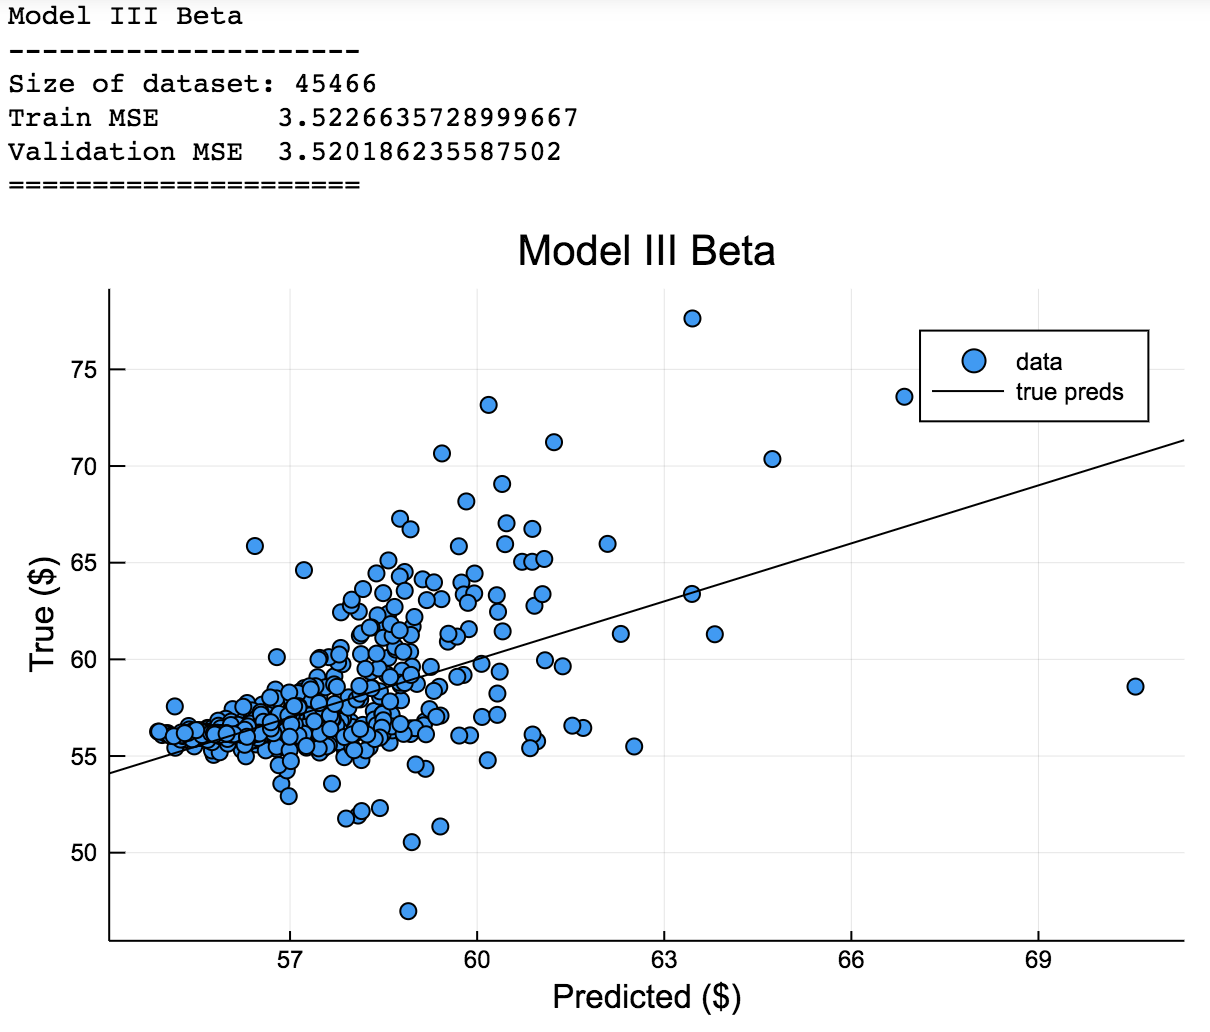
\includegraphics[width=.85\linewidth]{model3beta.png}
%      \caption{Model 3 Beta}
%   \end{minipage}
\end{figure}
\FloatBarrier
\subsubsection{Model III Beta has least Test Error}
% \begin{wrapfigure}{R}{0.3\textwidth}
% \centering
% 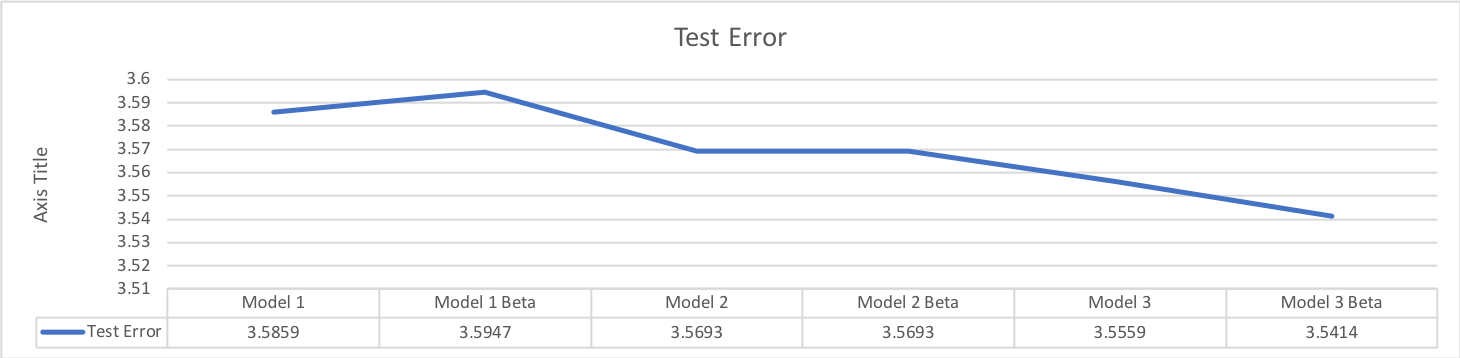
\includegraphics[width=0.3\textwidth]{Picture1.png}
% \caption{Single Feature}
% \end{wrapfigure}\par
% \begin{figure}
%     \centering
%     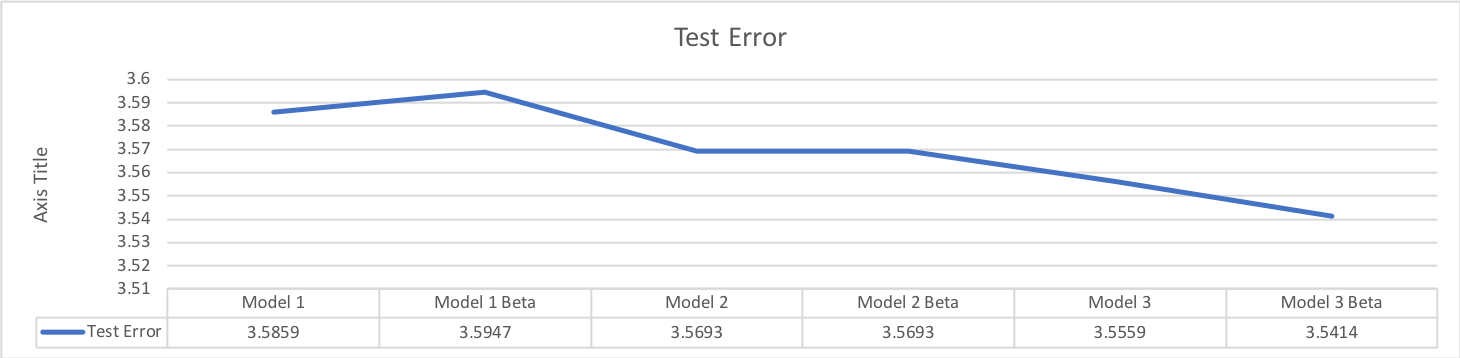
\includegraphics[scale =0.4]{Picture1.png}
%     \caption{Test Error}
%     \label{fig:my_label}
% \end{figure}
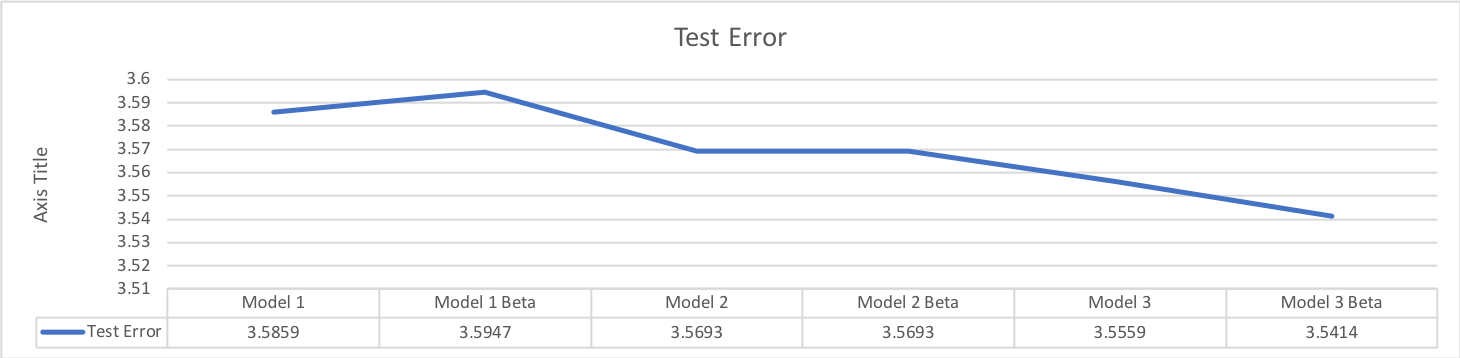
\includegraphics[scale =0.4]{Picture1.png}
\section{Future Plans}
The next step we are planning to do is to observe text data such as moive name and movie overview. Our initial thoughts is to do a \texttt{word2vec} embedding, and do a few computations and model training on that. We are also planning to use more complicated models such as Logisic Regression to train models.
\end{document}
